% -----------------------------------------------------------------------------
% Template from
% https://it.overleaf.com/articles/the-parallelization-and-optimization-of-the-n-body-problem-using-openmp-and-cuda/jpkcgbptkvby
% -----------------------------------------------------------------------------
\documentclass[letterpaper, 10 pt, conference]{ieeeconf}
\IEEEoverridecommandlockouts                              % This command is only
% needed if you want to
% use the \thanks command
\overrideIEEEmargins
% See the \addtolength command later in the file to balance the column lengths
% on the last page of the document


% The following packages can be found on http:\\www.ctan.org
\usepackage{graphics} % for pdf, bitmapped graphics files
\usepackage{epsfig} % for postscript graphics files
%\usepackage{mathptmx} % assumes new font selection scheme installed
%\usepackage{times} % assumes new font selection scheme installed
\usepackage{amsmath} % assumes amsmath package installed
\usepackage{amssymb}  % assumes amsmath package installed

\usepackage{url}
%\usepackage{algorithm}
\usepackage{verbatim}
%\usepackage[noend]{algpseudocode}
\usepackage{soul, color}
\usepackage{lmodern}
\usepackage{fancyhdr}
\usepackage[utf8]{inputenc}
\usepackage{fourier}
\usepackage{array}
\usepackage{makecell}

\renewcommand\theadalign{bc}
\renewcommand\theadfont{\bfseries}
\renewcommand\theadgape{\Gape[4pt]}
\renewcommand\cellgape{\Gape[4pt]}

\newcommand{\rework}[1]{\todo[color=yellow,inline]{#1}}

\makeatletter
\newcommand{\rom}[1]{\romannumeral #1}
\newcommand{\Rom}[1]{\expandafter\@slowromancap\romannumeral #1@}
\makeatother

\pagestyle{plain}

\title{\LARGE \bf
The Parallelization and Optimization of the N-Body Problem using OpenMP and CUDA
}

%\author{ \parbox{3 in}{\centering Huibert Kwakernaak*
%         \thanks{*Use the $\backslash$thanks command to put information here}\\
%         Faculty of Electrical Engineering, Mathematics and Computer Science\\
%         University of Twente\\
%         7500 AE Enschede, The Netherlands\\
%         {\tt\small h.kwakernaak@autsubmit.com}}
%         \hspace*{ 0.5 in}
%         \parbox{3 in}{ \centering Pradeep Misra**
%         \thanks{**The footnote marks may be inserted manually}\\
%        Department of Electrical Engineering \\
%         Wright State University\\
%         Dayton, OH 45435, USA\\
%         {\tt\small pmisra@cs.wright.edu}}
%}

\author{Tushaar Gangarapu, Himadri Pal, Pratyush Prakash and Suraj Hegde% <-this % stops a space 
\\ Department of Information Technology \\
National Institute of Technology Karnataka \\
Surathkal, Mangaluru 575025, Karnataka, India \\
{\tt\small\{tushaargvsg45, himadripal37, pratyushprakash47, suraj1997pisces\}@gmail.com} \\ \\
Dr. Geetha V%
\\ Department of Information Technology \\
National Institute of Technology Karnataka \\
Surathkal, Mangaluru 575025, Karnataka, India \\
{\tt\small geethav@nitk.edu.in}
}


\begin{document}


    \maketitle
    \thispagestyle{plain}
    \pagestyle{plain}


%%%%%%%%%%%%%%%%%%%%%%%%%%%%%%%%%%%%%%%%%%%%%%%%%%%%%%%%%%%%%%%%%%%%%%%%%%%%%%%%
    \begin{abstract}

        This research paper aims at exploiting efficient ways of implementing the N-Body problem. The N-Body problem, in the field of physics, predicts the movements and planets and their gravitational interactions. In this paper, the efficient execution of heavy computational work through usage of different cores in CPU and GPU is looked into; achieved by integrating the OpenMP parallelization API and the Nvidia CUDA into the code. The paper also aims at performance analysis of various algorithms used to solve the same problem. This research not only aids as an alternative to complex simulations but also for bigger data that requires work distribution and computationally expensive procedures.\\

    \end{abstract}

    \begin{keywords}

        N-Body, All-Pairs, Barnes-Hut, Parallelization, OpenMP, CUDA

    \end{keywords}

%%%%%%%%%%%%%%%%%%%%%%%%%%%%%%%%%%%%%%%%%%%%%%%%%%%%%%%%%%%%%%%%%%%%%%%%%%%%%%%%

    \section{INTRODUCTION}
    When the distribution of the train and test data differs, this is known as dataset shifting. This may produce several problems because the model is trained on one distribution but it is used to predict different data distributions, resulting in poorer results. There are different types of data shifting such as 
    Covariance Shift\footnote{Changes in the independent variables or features of the dataset},
    Probability Shift\footnote{Changes in the target variable or the dependent variable in the dataset}
    and Concept Shift.\footnote{Change in the connection between the independent and the target variable across datasets}
    In this work we analyze the presence of the Spatial Covariance Shift and try to address its main challenges.

    The data consists of pairs of meteorological features and target values at a particular latitude/longitude and time.
    The Regression task consist in predict the target value which is an air temperature measurements at 2 metres above the ground.
    The features are:
    \begin{itemize}
        \item \textit{weather-related features:} sun evaluation at the current location, climate values of temperature, pressure and topography, and meteorological parameters on different pressure
        \item \textit{surface levels} from weather forecast model predictions.
    \end{itemize} 
    Weather forecast model predictions are values produced by the following weather forecast models: 

    \begin{itemize}
        \item Global Forecast System \textit{(GFS)}
        \item Global Deterministic Forecast System from the Canadian Meteorological Center \textit{(CMC)}
        \item Weather Research and Forecasting \textit{(WRF) }
    \end{itemize}
    Each model returns the following predicted values: wind, humidity, pressure, clouds, precipitation, dew point, snow depth, air and soil temperature characteristics. Where applicable, the predictions are given at different isobaric levels from 50 hPa (20 km above ground) to the ground level.

    Altogether, there are 111 features in total. It is important to note that the features are highly heterogeneous, i.e., they are of different types and scales.

    The main challenge of this dataset is the Spatial Covariance Shift from train to test as is visible in Fig. \ref{fig:train-test-diff}

    \begin{figure}
        \centering
        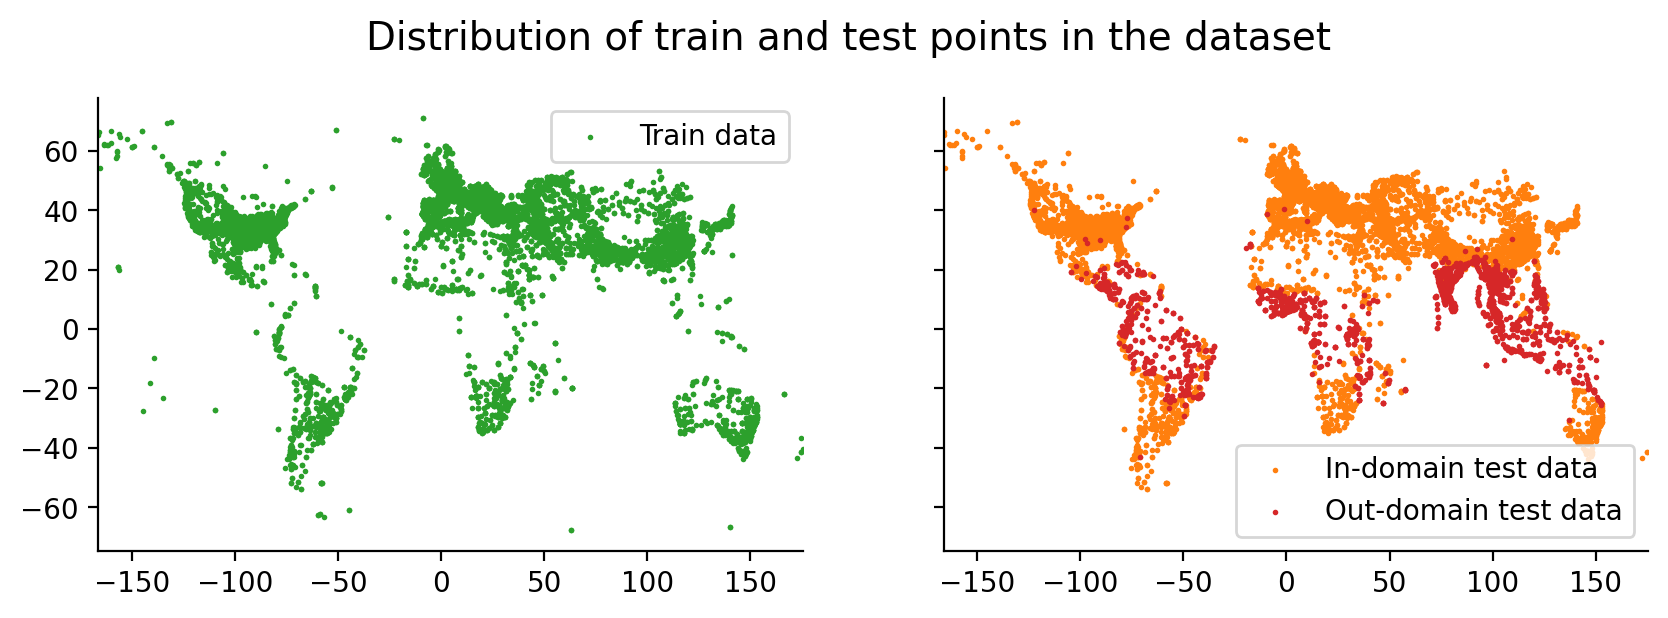
\includegraphics[width=\linewidth]{challenge1/assets/train-test-diff.png}
        \caption{The figure clearly shows that the regions in the range of latitude from -18 to 10 are not present in the train dataset. This phenomenon is called \textit{Spatial Covariance Shift}. [best visualization in colors] }
        \label{fig:train-test-diff}
    \end{figure}

    \section{LITERATURE SURVEY}

    \subsection{Background}

    The N-Body problem is concerned with the interactions between celestial bodies \cite{c5}, where every body in the given system of bodies is affected by every other body. The creation of galaxies, the effects of black holes and even the search for the dark matter are concerned with the N-Body problem. They all use Newton’s law of gravitation to show the effects on the motions of the bodies due to the forces of gravity acting between them.\par

    This project focuses on the celestial N-Body problem; with bodies interacting due to Newton’s Law of Gravitation. The N-Body problem can be described as follows: where N $\geq$ 2; For every i = 1,2, ...,N; let $B_i$ with mass $m_i$ be at $\vec{x}_i$, with velocity $\vec{v}_i$ and acceleration $\vec{a}_i$ at time t $\geq$ 0 and where $r_{ij}$ is the distance between $B_i$ and $B_j$; i $\neq$ j and $r_{ij}$ = $r_{ji}$ $\neq$ 0. The force acting on $B_i$ due to $B_j$ is $\vec{F}_{ij}$; a function of the distance between them ($r_{ij}$). Assume that $\vec{F}_{ij}$ = {--}$\vec{F}_{ji}$. Given initial positions and velocities of all $B_i$ $\forall$ i = 1, 2, ..., N; the general N-Body problem is to determine the motion of the system if each $B_i$ interacts with all other $B_j$’s in the system.

    \subsection{Literature Survey}

    In 1994, the Virgo Consortium was founded for the purpose of cosmological simulations on supercomputers. The largest problem worked on through the Virgo Consortium has been the Millennium Run \cite{c6}. It was created to model the formation of the universe and to track how galaxies and black holes are created. The simulation traced around 10 billion particles where each particle represented around 20 million galaxies. It used a code called \textit{GADGET}{--} GAlaxies with Dark matter and Gas intEract \cite{c7}, which was originally written in serial to model collisions between galaxies but has since been developed to run in parallel and is now used to model a larger range of astrophysical problems. \par

    The Virgo Consortium produces the \textit{GADGET} code along with \textit{MPI-HYDRA} and \textit{FLASH}. Although all codes are used to solve astrophysical N-body problems, they are used to simulate different areas. \textit{MPI-HYDRA} looks at galaxy formation, star formation and the x-ray transmission due to the heating and cooling of galaxies. \textit{FLASH} simulates the thermonuclear flashes seen on the surface of compact stars such as neutron stars and white dwarfs.


    \section{N-BODY PROBLEM}

    \subsection{Sequential All-Pairs Algorithm}

    The gravitational N-Body problem relies on two of Newton's Laws{--} Newton's Law of Gravitation, as in (\ref{eq:1}); two bodies, $B_i$ and $B_j$ of mass $m_i$ and $m_j$ are attracted to each other by a force $\vec{F}_{ij}$, which is inversely proportional to the square of the distance between them, $r_{ij}$ \textit{(G is Universal Gravitational Constant)} and Newton's Second Law of Motion, as in (\ref{eq:2}); a body, $B_i$, of mass $m_i$ will experience an acceleration, $\vec{a}_i$, if it experiences a force of magnitude $\vec{F}_i$ (force due to all the bodies in the system, \(\sum_{j \neq i}\vec{F}_{ij}\)).

    \begin{equation}
        \label{eq:1}
        \vec{F}_{ij} = \frac{Gm_im_j}{r_{ij}^2} \: \hat{\vec{r}}_{ij}
    \end{equation}

    \begin{equation}
        \label{eq:2}
        \vec{a}_i = \frac{\vec{F}_i}{m_i}
    \end{equation}

    Equations (\ref{eq:1}) and (\ref{eq:2}) can be combined to give (\ref{eq:3}). The acceleration $\vec{a}_i$ can be resolved direction wise as in (\ref{eq:4}) and (\ref{eq:5}). (Here we have considered N-Body problem in 2D.)

    \begin{equation}
        \label{eq:3}
        \vec{a}_i = \frac{Gm_j}{r_{ij}^2} \:
        \hat{\vec{r}}_{ij}
    \end{equation}

    \begin{equation}
        \label{eq:4}
        \vec{a}_{i, x} = \frac{Gm_j}{r_{ij}^2} \:
        \frac{x_i - x_j}{r_{ij}}
    \end{equation}

    \begin{equation}
        \label{eq:5}
        \vec{a}_{i, y} = \frac{Gm_j}{r_{ij}^2} \:
        \frac{y_i - y_j}{r_{ij}}
    \end{equation}

    Algorithm 1 given below is the serial All-Pairs algorithm used to compute forces on all bodies as explained above.

    \subsection{Parallelization of All-Pairs Algorithm (OpenMP)}

    The brute force algorithm is very easily parallelized as it is known in advance exactly how much work needs to be done. The work can be partitioned easily among processes with a block partitioning strategy. The number of bodies is known and to update each body takes the same amount of calculation. Assigning each process to calculate a block of bodies each $\frac{number of planets}{number of processors}$ in size will mean each process performs the same amount of calculations. Therefore partitioning the workload effectively; depicted by Algorithm 2.

    \subsection{Parallelization of All-Pairs Algorithm (CUDA)}

    Algorithm 3 given below is the parallel All-Pairs algorithm used to compute forces on all bodies using Nvidia CUDA.

    \subsection{Sequential Barnes-Hut Algorithm}

    The Barnes-Hut algorithm \cite{c8} approximates a solution to the gravitational N-Body problem by clustering groups of distant bodies together as a single pseudo-body. Each has an overall mass and center of mass based on the individual bodies it contains. It achieves this by creating a tree structure where each node has four children and each node has a center of mass and total mass based on that of its children. When created, this tree describes the whole system where each internal node represents a pseudo-body. Each star then uses the tree to work out the forces it experiences. The algorithm to realize the spatial system into a tree structure is achieved as follows:

    \begin{itemize}
        \item Divide the whole domain into four square regions of equal size.
        \item If any of these regions contains more than one body, recursively divide that region into four more squares. Continue until each square contains maximum of one body.
        \item Once the tree is created perform a recursive walk to calculate the center of mass, $\vec{c}$, as in (\ref{eq:6}), where $m_i$ is the mass of a node\'{}s $i^{th}$ child and $\vec{c}_i$ is the center of mass of a node\'{}s $i^{th}$ child.
        .

        \begin{equation}
            \label{eq:6}
            \vec{c} = \frac{\sum_{1}^i\vec{c}_im_i}{\sum_{1}^im_i}
        \end{equation}
    \end{itemize}


    This creates a tree where the root node (Fig. 1) contains the whole system. Each node has four children (Fig. 2) and the leaves of the tree are the individual bodies \cite{c9}. The construction of the tree can be done with  \(O(N\log(N))\) runtime. Each body now uses this tree to calculate the acceleration it experiences due to every other body. The force calculation is performed for each body. It recursively finds nodes in the tree which are considered to be far enough away to perform an interaction with. The calculation to decide whether a node is far enough away is called the \textit{opening condition}. It is important because it decides how many bodies can be grouped together as a pseudo-body; the more bodies which are grouped together, the less accurate the calculations will be. The opening condition is a simple relationship, \(\frac{l}{D} < \theta\), where \(\theta\) is the fixed accuracy parameter which is positive, l is the width of the current internal node and D is the distance of the body from the center of of mass of the current node to the body the force is being calculated for. The sequential algorithm for the same is given as Algorithm 4.

    \subsection{Parallel Barnes-Hut Algorithm using OpenMP{--} Force Computation is Parallelized (Method-1)}

    Two major issues involved in the analysis of a parallel algorithm include \textit{Decomposition}{--} divide the problem amongst available processes and \textit{Communication}{--} need to communicate between processes to assure they have data they need. Decomposition is associated with load balancing while Communication bottleneck is a major issue; need for minimization of communication volume. Barnes-Hut algorithm construction is as follows:

    \begin{itemize}
        \item Build the quad-tree.
        \item Calculate the center of mass for all cells.
        \item Traverse the quad-tree.
        \item Calculate the force on the nodes.
    \end{itemize}

    Building the quad-tree needs synchronization. Since the computation of the center of mass depends on the center of masses of corresponding sub-cells, data dependencies are introduced{--} can be parallelized per level. To compute the force, we need other particles' center of mass, but we don't need to modify this information{--} can be parallelized. The value of $\theta$ plays a crucial role- a higher value of $\theta$ implies that fewer nodes are considered for the calculation of force and hence increasing the window for error. Algorithm 5 given below, depicts the parallelized version of Barnes-Hut algorithm in the way described above.

    \subsection{Parallel Barnes-Hut Algorithm using OpenMP{--} Mass Distribution is Parallelized (Method-2)}

    In computing the center of mass of the nodes, even though the presence of data level dependencies restricts parallelizing, some level of parallelism can still be introduced as the computation done for each quad is independent of the other. So, all these computations can occur in parallel; this speeds up the process significantly. So, in the Algorithm-6 described below only the center of mass computation has been parallelized leaving the force computation as it is. The graphs plotted have been shown in the sections that follow. \par

    Parallelization of the Barnes-Hut algorithm has many issues making it more complex than anything so far seen in this project. The main issue is the lack of prescience of the number of calculations done by each process. With the increase in the tree traversal depth, the number of force calculations increase and the exact depth is dependent on the position of the current body, which is random.


    \section{WORK DONE AND RESULTS ANALYSIS}

    The sequential All-Pairs algorithm is implemented in C++. The parallelization of the algorithm is performed using OpenMP and CUDA. OpenMP is a usage of multi-threading \cite{c11}; an expert string forks a predetermined number of slave strings and the framework separates an errand among them. The strings then run simultaneously, with the runtime environment assigning strings to distinctive processors. The segment of code that is intended to keep running in parallel is stamped likewise, with a preprocessor order that will bring about the strings to shape before the segment is executed. Each string has an \textit{id} appended to it which can be acquired utilizing a method \textit{omp\_get\_thread\_num()}. After the execution of the parallelized code, the strings join over into the master string, which proceeds with forward to the end of the system. \par

    CUDA is an extension of the C that allows the programmer to take advantage of the massive parallel computing power of an Nvidia graphics card in order to do general purpose computation \cite{c12}. In order to run efficiently on a GPU, you need to have many hundreds of threads. Generally, the more threads you have, the better.If you can break the problem down into at least a thousand threads, then CUDA probably is the best solution. When something extremely computationally intense is needed, the problem can simply call the CUDA kernel function written by the user. GPUs use massive parallel interfaces in order to connect with it’s memory; is approximately 10 times faster than a typical CPU to memory interface. \par

    This section focuses on running each algorithm in serial and in parallel. Testing Speedup, Cost and Efficiency (see equations (\ref{eq:7}), (\ref{eq:8}), (\ref{eq:9})). All the tests for All-Pairs algorithm (openMP) are ran on nearly identical machines with the following specification:
    \begin{itemize}
        \item Model{--} Asus
        \item Processor{--} i5 7200U @ 4x 3.1GHz
        \item Memory{--} 8GB DDR3 at 1333MHz
        \item Network{--} 10/100/1000 Gigabit LAN Connection
        \item Operating System{--} Arch Linux
    \end{itemize}

    All the tests for All-Pairs algorithm (CUDA) are ran on nearly identical machines with the following specification:
    \begin{itemize}
        \item Nvidia Tesla Server
        \item Operating System{--} Ubuntu Linux
    \end{itemize}

    All the tests for Barnes-Hut algorithm (openMP, both methods) are ran on nearly identical machines with the following specification:
    \begin{itemize}
        \item Model{--} HP
        \item Processor{--} i5 6200U
        \item Memory{--} 8GB DDR3 @ 2.8GHz
        \item Network{--} 10/100/1000 Gigabit LAN Connection
        \item Operating System{--} Ubuntu Linux
    \end{itemize}

    \begin{equation}
        \label{eq:7}
        Speedup (S) = \frac{Time for Serial Execution}{Time for Parallel Execution}
    \end{equation}

    \begin{multline}
        \label{eq:8}
        Cost (C) = Parallel Execution \\
        \times Number of Processors
    \end{multline}

    \begin{equation}
        \label{eq:9}
        Efficiency (E) = \frac{Speedup}{Time for Parallel Execution}
    \end{equation}

    \subsection{Result and Analysis of Parallel All-Pairs algorithm in OpenMP and Nvidia CUDA}



    For inputs with a small number of planets we find sequential execution to be faster than parallelized OpenMP code (Fig. 3). This supports the fact that threads have a high cost of initialization, which outweighs the execution time since it is smaller in comparison. When we increase the input size, the parallel code runs much faster than the sequential counterpart. Since the input is large, the time of execution is also larger than the tread spawn overheads. (Fig. 4). However we notice that increasing the threads beyond a certain value does not cause any further decrease. This is because the CPU on the test machine cannot support more than 4 threads. Therefore we see a flat curve after. For an input file with very large inputs the graph remains the same as the previous graph. However there is a larger speedup (Fig. 5). \par

    From Figures 3, 4 and 5 we observe that there is a large speedup for input files with a large size and this speedup is limited to the number of threads on the test machine. For small inputs, sequential execution remains faster than parallelization with OpenMP. In the case of parallelization with CUDA, we see an exponential decrease in CUDA time. This follows from the fact that the GPU has an exponentially larger thread pool as compared to the CPU (Figures 6, 7, 8). \par

    For a very small input the communication over PCI lanes is the bottleneck as execution time is negligible. Hence we see that sequential is comparable to the CUDA program. In the case of Fig. 6 we find parallel execution with CUDA an order of 100 times faster than sequential. As the number of threads per block is increased beyond a certain value the execution time decreases drastically. Fig. 8 shows CUDA execution times for an input file of very large size. The speedup of CUDA with 2048 threads per block over sequential is approximately 350. This means with heavy parallelization of the GPU, we can achieve the results much quicker than doing the same on the CPU. This confirms the fact that GPUs typically have more multiprocessing capabilities than the CPU.

    \subsection{Result and Analysis of Parallel Barnes-Hut Algorithm using OpenMP}

    In Fig.9, the sequential algorithm proved to be efficient as compared to OpenMP. One explanation for the same would include the communication overhead and thread overhead for such small dataset (5 bodies). In Fig. 10, it was observed that the OpenMP implementation performed better in the case of 2 and 4 threads but the overheads increased as the number of threads increased from 4. In the case of Fig. 11, the Barnes-Hut implementation in OpenMP algorithm performed better in the case of 2 threads but increased progressively before reducing once in 8 threads and increasing again. \par

    In Fig. 12, the time reduced drastically for 8 threads and above. Although, an anomaly was observed for 4 threads. In case of Fig. 13, it was observed that for \textit{galaxy30k} performed better than the sequential for 4 and 8 threads and then increased linearly with the number threads, again changing the trend from 16 threads onwards. As observed in Fig. 14 for \textit{planets.txt} the overhead increases progressively. Hence, we can infer that the dataset \textit{planets.txt} has data which does not go well with the tree building methodology. \par

    The value of $\theta$ determines how deep the Barnes-Hut algorithm traverses the tree. The smaller the value the deeper it goes, increasing accuracy but at the cost of an increased number of calculations and therefore a slower running time. Experimentally it can be seen that as $\theta$ tends to 0 the number of calculations increases, as expected. As $\theta$ reaches 0.3 the number of calculations begin to rise quickly and at 0.1 the larger problems have to computer many more calculations. When $\theta$ is 0 the number of calculations is equal to the number of bodies in the set. This shows the algorithm has become just as complex as the All-Pairs method, with each body needing to calculate forces due to every other star.


    \section{CONCLUSIONS}

    In this paper, we analyzed two algorithms to solve the classical N-Body problem{--} the naive All-Pairs Algorithm and quad-tree based Barnes-Hut Algorithm in OpenMP and CUDA. Compared to the sequential execution we noticed a decrease in execution time till a certain level of parallelization, after which the time either remained the same or increased. The performance of these algorithms can be further bettered by running the algorithms on a processor with a higher multiprogramming support. \par

    The parallel direct method scaled linearly with respect to the number of processes. The communication overhead for the parallel direct method is negligible as the number of stars is so small, but as more processes are added the algorithm becomes plausible for larger numbers of N, but with increasing N will come increasing communication overheads. Due to limitations with time this project only implemented a simple parallel version of the Barnes-Hut algorithm that contains no load balancing. The computation time of the Parallel Barnes-Hut scaled almost linearly, but with an increasing number of processes came an increasing communication overhead which soon outweighed the benefit seen due to the increase in computation time. The Barnes-Hut algorithm can offer substantial increases in running time depending on the choice of $\theta$. This shows how well the naive method is improved by parallel computing.


    \addtolength{\textheight}{-12cm}   % This command serves to balance the column lengths
    % on the last page of the document manually. It shortens
    % the textheight of the last page by a suitable amount.
    % This command does not take effect until the next page
    % so it should come on the page before the last. Make
    % sure that you do not shorten the textheight too much.

%%%%%%%%%%%%%%%%%%%%%%%%%%%%%%%%%%%%%%%%%%%%%%%%%%%%%%%%%%%%%%%%%%%%%%%%%%%%%%%%


%%%%%%%%%%%%%%%%%%%%%%%%%%%%%%%%%%%%%%%%%%%%%%%%%%%%%%%%%%%%%%%%%%%%%%%%%%%%%%%%


%%%%%%%%%%%%%%%%%%%%%%%%%%%%%%%%%%%%%%%%%%%%%%%%%%%%%%%%%%%%%%%%%%%%%%%%%%%%%%%%
    \section*{APPENDIX}

    The appendix shows the analysis of the Barnes-Hut algorithm implemented in Parallel using OpenMP (method-1). The Sequential and Parallel times have been shown in Table 1; for all the galactic datasets \cite{c4} with number of bodies ranging from 5 to 30002.

    \begin{table*}[h]
        \caption{Performance of Serial Code vs. Parallel Code on galactic datasets \cite{c4} of Barnes-Hut Algorithm in OpenMP (Method-1)}
        \label{tab:1}
        \begin{center}
            \begin{tabular}{|c||c||c||c||c||c||c||c||c|}
                \hline
                \thead{Dataset} & \thead{Number of Particles} & \thead{Serial Time \\ (seconds)} & \multicolumn{6}{l|}{\thead{Parallel Time (seconds)}} \\
                \cline{4-9}
                &       &           & \multicolumn{6}{l|}{\thead{Number of Threads}} \\
                \cline{4-9}
                &  &  & \thead{1}  & \thead{2}  & \thead{4}  & \thead{8}  & \thead{16}   & \thead{32}   \\
                \hline
                asteroids1000.txt    & 1000  & 0.023097  & 0.020348  & 0.021905  & 0.030464  & 0.063325  & 0.121116   & 0.221256   \\
                \hline
                cluster2582.txt     & 2582  & 0.004927  & 0.005837  & 0.005042  & 0.011231  & 0.008328  & 0.011733   & 0.014243   \\
                \hline
                collision1.txt     & 2000  & 0.004917  & 0.004829  & 0.004447  & 0.006030  & 0.005751  & 0.009468   & 0.012608   \\
                \hline
                collision2.txt        & 2002   & 0.006227  & 0.006008  & 0.006098  & 0.006309  & 0.006821  & 0.009951   & 0.013182   \\
                \hline
                galaxy1.txt        & 802   & 0.015414  & 0.015616  & 0.015217  & 0.020928  & 0.045315  & 0.072090   & 0.110689   \\
                \hline
                galaxy2.txt        & 652  & 0.012274  & 0.012615  & 0.014664  & 0.023931  & 0.028826  & 0.040485   & 0.072064   \\
                \hline
                galaxy3.txt        & 2001   & 0.091639  & 0.087738  & 0.094466  & 0.141264  & 0.264529  & 0.488200   & 0.975077   \\
                \hline
                galaxy4.txt      & 502 & 0.012875  & 0.013325  & 0.010431  & 0.012065  & 0.027304  & 0.037397  & 0.051786  \\
                \hline
                galaxy10k.txt      & 10001 & 2.325312 & 2.357691 & 2.422882 & 3.557520 & 6.697054 & 13.312913  & 27.061886 \\
                \hline
                galaxy20k.txt      & 20001 & 13.663441  & 15.492622  & 16.259973  & 23.813991  & 45.588013  & 88.301931   & 160.741782   \\
                \hline
                galaxy30k.txt & 30002  & 0.032405  & 0.032411  & 0.031647  & 0.057545  & 0.050811  & 0.075314   & 0.171779   \\
                \hline
                galaxyform2500.txt   & 2500  & 0.007052  & 0.005922  & 0.006162  & 0.006707  & 0.008641  & 0.011501   & 0.016563   \\
                \hline
                galaxymerge1.txt   & 2000  & 0.004920  & 0.005160  & 0.004812  & 0.006784  & 0.006742  & 0.008701   & 0.018789   \\
                \hline
                galaxymerge2.txt   & 4000  & 0.011205  & 0.010364  & 0.003930  & 0.012193  & 0.011976  & 0.018860   & 0.024891   \\
                \hline
                galaxymerge3.txt        & 2901     & 0.009433  & 0.009095  & 0.009045  & 0.015460  & 0.011692  & 0.012852   & 0.019202   \\
                \hline
                planets.txt    & 5 & 0.000070  & 0.000120  & 0.000406  & 0.001250  & 0.001246  & 0.001997   & 0.003918   \\
                \hline
                saturnrings.txt   & 11987   & 0.024471  & 0.024749  & 0.020095  & 0.025863  & 0.032043  & 0.038763   & 0.064468   \\
                \hline
                spiralgalaxy.txt   & 843   & 0.017879  & 0.017627  & 0.023605  & 0.024740  & 0.052584  & 0.091534   & 0.166260   \\
                \hline
            \end{tabular}
        \end{center}
    \end{table*}

    \section*{ACKNOWLEDGMENT}

    We would like to thank Dr. Geetha V for her valuable comments and suggestions to improve the
    quality of the paper. We are also grateful to Miss Archana for helping us review our work regularly. We would also like to thank the Department of Information Technology, NITK Surathkal for providing us with Tesla GPU for us to test our code.


%%%%%%%%%%%%%%%%%%%%%%%%%%%%%%%%%%%%%%%%%%%%%%%%%%%%%%%%%%%%%%%%%%%%%%%%%%%%%%%%

\end{document}